\begin{center}
	\LARGE
	Bag en kage
\end{center}

I skal i denne aflevering bage en kage. Det må være i netværksgrupper eller grupper af eget valg. Mængden af ingredienser skal I finde ved at løse en række opgaver. Opskriften er på en gulerodskage med cream cheese frosting tyvstjålet fra en ikke nærmere bestemt, men ganske udbredt dansk madblogger.

\textbf{Ingredienser til kagen}
\begin{itemize}
	\item[$\cdot$] \underline{\phantom{150}} g stuetempereret smør.
	\item[$\cdot$] \underline{\phantom{100}} g sukker.
	\item[$\cdot$] \underline{\phantom{100}} g brun farin.
	\item[$\cdot$] \underline{\phantom{4}} æg.
	\item[$\cdot$] \underline{\phantom{200}} g hvedemel.
	\item[$\cdot$] \underline{\phantom{2}} tsk bagepulver.
	\item[$\cdot$] \underline{\phantom{1}} tsk kanel.
	\item[$\cdot$] \underline{\phantom{0.5}} tsk salt.
	\item[$\cdot$] \underline{\phantom{275}} g skraldede og groftrevne gulerødder.
\end{itemize}

\textbf{Ingredienser til topping}
\begin{itemize}
	\item[$\cdot$] \underline{\phantom{125}} g stuetempereret smør.
	\item[$\cdot$] \underline{\phantom{1}} tsk vaniljesukker 
	\item[$\cdot$] \underline{\phantom{125}} g flormelis.
	\item[$\cdot$] \underline{\phantom{125}} g naturel flødeost.
	\item[$\cdot$] Saft og skal fra \underline{\phantom{1}} økologisk citron.
\end{itemize}

\textbf{Fremgangsmåde til kage}
Pisk smør, sukker og brun farin luftigt. Pisk derefter ét æg i ad gangen, så blandingen ikke skiller. 

Bland de tørre ingredienser godt sammen i en anden skål og vend herefter de tørre ingredienser i dejen. Vend til sidst den revne gulerod i dejen og bag kagen i en smurt springform på 20cm diameter ved 170$^\circ$C varmluft i ca. 45 minutter. 

\textbf{Fremgangsmåde til frosting}
Pisk smør, sukker og vaniljesukker sammen til det er luftigt. Bland citronsaft, citronskal og flødeost i blandingen og smør den på kagen, når kagen er helt kold. 

\newpage

\begin{opgavetekst}{Opgave 1}
	En vektor $\vv{a}$ er givet ved
	\begin{align*}
		\vv{a} = 
		\begin{pmatrix}
			200 \\
			a_2
		\end{pmatrix}.
	\end{align*}
\end{opgavetekst}	
\begin{delopgave}{1}
	Bestem tallet $a_2$ så længden af $\vv{a}$ er $250$.
\end{delopgave}
\begin{delopgave}{2}
	Bestem prikproduktet mellem $\vv{a}$ og vektoren $\vv{b}$ givet ved
	\begin{align*}
		\vv{b} = 
		\begin{pmatrix}
			10 \\
			\frac{-38}{3}
		\end{pmatrix}.
	\end{align*}
\end{delopgave}

\begin{opgavetekst}{Opgave 2}
	To linjer $l$ og $m$ er givet ved henholdsvis
	\begin{align*}
		&l: \ 2(x- 5) + \frac{9}{2}(y + 1) = 0\\
		&m: \ \frac{2}{5}(x+1) -\frac{1}{10}(y-12) = 0
	\end{align*}
\end{opgavetekst}
\begin{delopgave}{1}
	Bestem den stumpe vinkel mellem $l$ og $m$. 
\end{delopgave}
\begin{meretekst}
	En linje $n$ er givet ved parameterfremstillingen	
	\begin{align*}
		n: \ 
		\begin{pmatrix}
			x \\ y
		\end{pmatrix}
		=
		\begin{pmatrix}
			5 \\ -1
		\end{pmatrix} 
		+
		t
		\begin{pmatrix}
			-9 \\ k
		\end{pmatrix}
	\end{align*}
\end{meretekst}
\begin{delopgave}{2}
	Bestem tallet $k$ så linjerne $n$ og $l$ er parallelle. 
\end{delopgave}

\begin{opgavetekst}{Opgave 3}
	Grafen for en funktion $g$ givet ved
	\begin{align*}
		g(x) = -x^2 + 10x + \frac{19}{3}
	\end{align*}
	kan ses på Figur \ref{fig:opg3}.
	\begin{figure}[H]
	\centering
	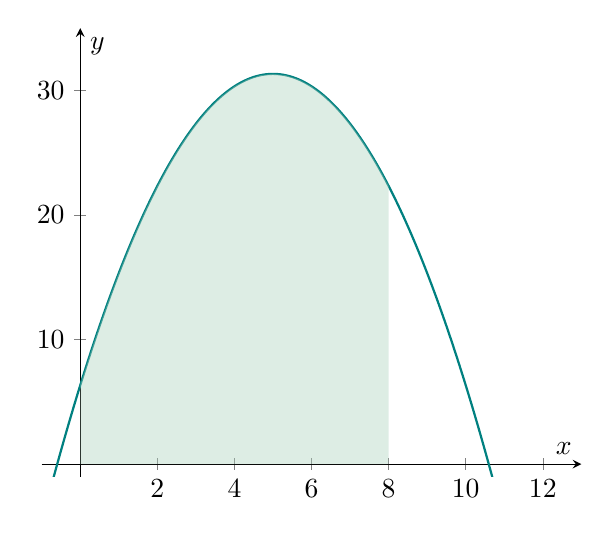
\begin{tikzpicture}
	\begin{axis}[
		axis lines = center, 
		xmin = -1, xmax = 13,
		ymin = -1, ymax = 35,
		xtick = {-2,0,2,...,14,16},
		xlabel = $x$, 
		ylabel = $y$, 
	]
		\addplot[color = teal, thick, domain = -1:13, samples = 300] {-x^2+10*x+19/3};	
		\fill
		[
			color = SeaGreen!40,
			opacity = 0.4,
			variable = \x, 
			domain = 8:0,
		]	
			(axis cs: 0,0) -- (axis cs: 8,0) --
			plot(axis cs: \x, {-(\x)^2 + 10*\x + 19/3}) --  cycle;
	\end{axis}
	\end{tikzpicture}
	\caption{Areal under $f$.}
	\label{fig:opg3}
	\end{figure}
	\phantom{h}
\end{opgavetekst}
\begin{delopgave}{1}
	Bestem arealet af det skraverede område på Figur \ref{fig:opg3}.
\end{delopgave}
\begin{meretekst}
	Grafen for funktionen $h$ givet ved
	\begin{align*}
		h(x) = x^2 + bx + 5 
	\end{align*}
	afgrænser sammen med funktionen $g$ et areal på $\frac{52}{3}$ på intervallet $[1,3]$. 
\end{meretekst}
\begin{delopgave}{2}
	Bestem tallet $b$.
\end{delopgave}

\begin{opgavetekst}{Opgave 4}
	En funktion $f$ er givet ved
	\begin{align*}
		f(x) = \ln(2x-4).
	\end{align*}
\end{opgavetekst}
\begin{delopgave}{1}
	Bestem $f'(3)$. 
\end{delopgave}

\begin{opgavetekst}{Opgave 5}
	En funktion $g$ er givet ved
	\begin{align*}
		g(x) = \sqrt{x^2-x+4}
	\end{align*}
\end{opgavetekst}
\begin{delopgave}{1}
	Bestem ekstremumsstedet for $g$. 
\end{delopgave}


\begin{opgavetekst}{Opgave 6}
	En trekant $\triangle ABC$ opfylder, at $a = 77$, $b = 231$ og $\angle C = 117.33^\circ$.
\end{opgavetekst}
\begin{delopgave}{1}
	Bestem længden $c$.
\end{delopgave}

\begin{opgavetekst}{Opgave 7}
	To vektorer $\vv{u}$ og $\vv{v}$ er givet ved
	\begin{align*}
		&\vv{u} = 
		\begin{pmatrix}
			5 \\ 4
		\end{pmatrix}, &
		&\vv{v} = 
		\begin{pmatrix}
			7.5 \\
			-19
		\end{pmatrix}
	\end{align*}
\end{opgavetekst}
\begin{delopgave}{1}
	Bestem arealet af det parallelogram, der udspændes af vektorerne $\vv{u}$ og $\vv{v}$. 
\end{delopgave}

\begin{opgavetekst}{Opgave 8}
	En funktion $f$ har forskriften
	\begin{align*}
		f(x) = \sqrt{5x}.
	\end{align*}
\end{opgavetekst}
\begin{delopgave}{1}
	Hvor langt skal grafen for $f$ parallelforskydes til venstre for at gå gennem punktet $(4,5)$? 
\end{delopgave}
%
%
\begin{opgavetekst}{Opgave 9}
	I en bank får du en årlig rente på 2.8$\%$. Du indsætter $100\TS 000$ kr i banken.
\end{opgavetekst}
\begin{delopgave}{1}
	Hvor mange penge står på kontoen efter 8 år? Beløbet skal angives i 1000 kroner. 
\end{delopgave}
\begin{delopgave}{2}
	Efter hvor mange år vil der være $3 \TS 156 \TS 016$ kr på kontoen?
\end{delopgave}
%
%
\begin{opgavetekst}{Opgave 10}
	En stykvist defineret funktion $g$ er givet ved
	\begin{align*}
		g(x) = 
		\begin{cases}
			x^2 + 4x - 3,  &\textnormal{ hvis }x \leq 2,\\
			4x + b,  &\textnormal{ hvis }x > 2.
		\end{cases}
	\end{align*}
\end{opgavetekst}
\begin{delopgave}{1}
	Bestem tallet $b$, så grafen for $g$ er kontinuert? 
\end{delopgave}